% Software License Agreement
%
% Author    Chris Bogdon <cbogdon@clearpathrobotics.com>
% Copyright (c) 2015, Clearpath Robotics, Inc., All rights reserved.
%
% Redistribution and use in source and binary forms, with or without modification, is
% not permitted without the express permission of Clearpath Robotics.


\documentclass[]{clearpath-latex/clearpath-manual}
\graphicspath{{gen/}}
\usepackage{multirow}
\usepackage{gensymb}
\usepackage{dcolumn}
\usepackage{colortbl}
\usepackage{array}
\usepackage{hyperref}
\usepackage{fancyhdr}
\pagestyle{fancyplain}
\lfoot{Rev. 1.0.0}
\rfoot{Warthog}
\lhead{}
\chead{}
\rhead{}
\renewcommand{\headrulewidth}{0pt}


\begin{document}

\manualcover{cover-page.pdf}
\tableofcontents

\section{Introduction}
Clearpath Robotics Warthog is a rugged, all-terrain unmanned ground vehicle capable of traveling on land and in water.  Warthog fully supports the Robot Operating System (ROS) and can be equipped with a variety of payloads, including sensors and manipulators, to accomodate a wide variety of robotics applications in mining, agriculture and environmental monitoring. This guide contains information about the setup, safe operation, and maintenance of your Warthog unmanned ground vehicle (UGV).  Please read the entire manual and safety warnings prior to operating the Warthog.

\subsection{What's Included}

Included with each Warthog are the following:

\begin{itemize}[nolistsep]
  \item 1x Warthog Amphibious Robotic Platform
  \begin{itemize}
    \item{Onboard computer}
    \item{User Integration Area with power, Ethernet, Serial(RS232) and USB connectivity}
    \item{48V Lead Acid Battery Pack}
    \item{Battery Charger}
  \end{itemize}
  \item 1x Futaba Remote Control (R/C)
  \item 1x Warthog User Manual
  \item 1x Wireless Stop Remote
\end{itemize}



\pagebreak[4]
\subsection{Hardware Overview}

Please see \autoref{Warthog_overview} for a view of some of Warthog's key external-facing features.

\begin{figure}[h]
  \centering
  \includegraphics[width=1\linewidth]{Warthog_Rear_Drawing_Labeled.pdf}
  \caption{Warthog Hardware Overview}
  \label{Warthog_overview}
\end{figure}





\pagebreak[4]
\subsubsection{Battery Charger}
Info about battery charger

\subsubsection{Bilge Pump}
Two bilge pumps are installed in each Warthog UGV. There is one situated in each of the drive units underneath the motor.

The bilge pumps are used to remove water from the main chassis and drive units. At initial startup, an audible sound can be heard from the bilge pumps being initiated. These pumps are an automatic pumping system that check for water levels inside the drive units. The pumps automatically come on every two minutes and check for water levels. If the water level inside the drive unit exceeds a predetermined level, the pumps will remain on, otherwise they will shut off. During prolonged use in water, some water may appear in the drive unit. This is normal and acceptable.

<picture of pump from inside and outside>

This outlet leads from the pump to the exterior of the Warthog UGV. It is used to remove excess water from the chassis and drive units. No obstructions should be placed in front of or around this area. Obstruction of water flow may result in damage to the internal electrical components and loss of function in the Warthog UGV.

\subsubsection{User Integration Area}\label{userbay}

The User Bay provides access to the User Power panel, as well as USB, Serial, and Ethernet ports.  The electrical panel can be used to power your payloads. The USB3 and ethernet  ports are connected directly to the onboard PC. To connect a device to the onboard network, it's suggested to give it a static IP in the \lstinline{192.168.131.x} subnet, avoiding IPs in use by the following pre-existing devices:

\bgroup
\def\arraystretch{1.2}%
\begin{table}[h]
  \centering
  \begin{tabular}{>{\columncolor{lightgrey}}>{\raggedright}m{.3\textwidth} p{.65\textwidth}} \hline

  192.168.131.1 & Onboard PC (all ports, br0 network interface). \\ \hline

  192.168.131.2 & Ethernet-connected MCU. \\ \hline

  192.168.131.14 & Front-facing LIDAR (optional). \\ \hline

  192.168.131.13 & Rear-facing LIDAR (optional). \\ \hline

  \end{tabular}
\newline
\caption{Warthog Onboard Network Devices}
\label{netdevs}
\end{table}
\egroup

For more information on electrical integration, please see \autoref{electrical} on page \pageref{electrical}.


\subsubsection{Payload Integration Racks}

All payloads should be mounted to the central chassis when traversing through water to prevent rolling. The primary payload of the unit should be placed on the central chassis. If necessary loading can be placed on the drive units however, payloads should not exceed 50 lbs on each drive unit.

For more information and guidance on mounting payload structures on top of Warthog, please refer to \autoref{mechanical} on page \pageref{mechanical}.


\pagebreak[4]
\subsection{Technical Specifications}

Key specifications of Warthog are shown in \autoref{systemspecs}.

\bgroup
\def\arraystretch{1.2}%
\begin{table}[h]
  \centering
  \begin{tabular}{>{\columncolor{lightgrey}}>{\raggedright}m{.30\textwidth} p{.70\textwidth}} \hline

  External Dimensions (L x W x H) & 1.52 x 1.38 x 0.83 m (4.9 x 4.5 x 2.72 ft ) \\ \hline
  Base Weight & 280 kg (551 lbs) \\ \hline
  Ground Clearance & 254 mm (10 in) \\ \hline
  Max Payload  &  272 kg (600 lbs)   \\ \hline
  Max Incline & 35-45° \\ \hline
  Max Speed  &  18 km/h (11 mph) \\ \hline
  Suspension & Geometric Passive Articulation \\ \hline
  Drive Configuration &  4x4 Skid Steer \\ \hline
  Operating Environment  &  Outdoor \\ \hline
  Traction & 24" Argo tire (24" Turf tire or 12" wide Quad Track System optional) \\ \hline
  Battery Chemistry & AGM sealed lead acid (Li-ion optional) \\ \hline
  Capacity &  105 Ah at 48 V, expandable to 200 Ah with Li-ion option \\ \hline
  Nominal Run Time & Lead acid: 2.5 hrs, Li-ion: 6 hrs \\ \hline
  Charge Time &  4 Hours approx \\ \hline
  User Power & 5 V, 12 V Fused (24 V, 48 V optional) \\ \hline
  Control Modes & Remote control, computer controlled velocity commands, indoor/outdoor autonomy packages \\ \hline
  Feedback & Battery voltage, motor currents, wheel odometry, control system status, temperature, safety status \\ \hline
  Communication &  Ethernet, USB, Remote Control, Wi-Fi \\ \hline
  Drivers and APIs  &  Packaged with ROS Indigo (includes RViz, Gazebo support), Matlab API available \\ \hline

  \end{tabular}
\newline
\caption{Warthog System Specifications}
\label{systemspecs}
\end{table}
\egroup




\section{Getting Started}

The first step is read the manual and safety warnings.  The next step is to power up your Warthog and have some fun driving it around! If you’re just opening up the shipping crate and remove the ratchet straps which secure Warthog during shipping.

Twist the power button on the back of Warthog. Once the body lights are flashing red, clear the two stop buttons (if necessary), and press the blinking red stop reset button. In a moment, the platform should go to solid red lights in back, and solid white in front.

\subsection{Wireless Stop Remote}

Inclued with the Warthog, is a wireless stop remote which is needed for operateration as shown in Figure \autoref{wireless-stop} below.
If the wireless stop remote is out of range, it will cause the system to stop.
Likewise, if the wireless stop remote is inactive for 15 minutes, it will cause the system to stop.
To turn on the remote, hold down the red 'POWER' button untill the battery and signal strength flash.
The vehicle's lights will give an indication of the state of the stop system.
To assert a stop, simply press the 'Stop' button which will be verified by the Warthog's lights flashing red.
Similarly, to release the stop system, press 'Stop' followed by 'GO'.
Additionally, pressing and holding 'GO' down for 5 seconds stopped or not, will initiate a power down of the on-board computer.

\begin{figure}[!h]
  \centering
  \includegraphics[width=1.0\linewidth]{wireless-stop-remote.png}
  \caption{Warthog's Wireless Stop Remote}
  \label{wireless-stop}
\end{figure}


If you’re not seeing any action, check Contact on \autoref{contact} to get in touch with support.

\subsection{Futaba Controller}

The long range remote control (RC) Futaba radio transmitter can be used to tele-operate the Warthog.
To begin, slide the power switch to the on position which is labelled in Figure \autoref{fubata}.
Caution, the speed adjustment knob should be turned initially all the way to the left while familiarizing yourself with the transmitter and slowly increasing it to get it moving.
The position of the speed adjustment scale is shown in  \autoref{futaba-screen} as 'CH4'.
The transmitter needs to be enabled which is done using the Enable/Disable switch that is a three position switch where only the down position enables it.
The left joy stick is used for the forward and reverse motion of the robot and the right is used for turning.



\begin{figure}[!h]
  \centering
  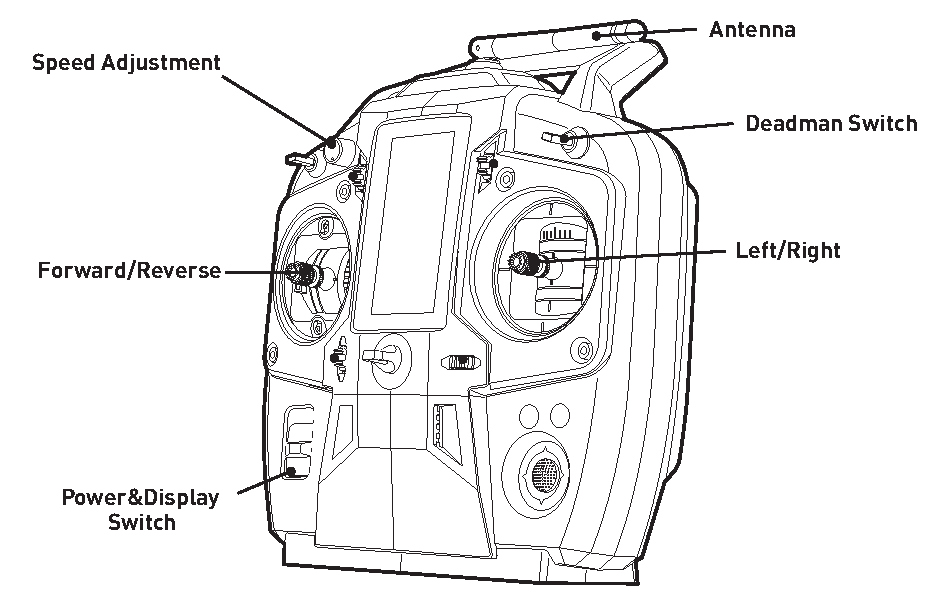
\includegraphics[width=1.0\linewidth]{futaba.pdf}
  \caption{Futaba Radio Transmitter}
  \label{futaba}
\end{figure}

\begin{figure}[!h]
  \centering
  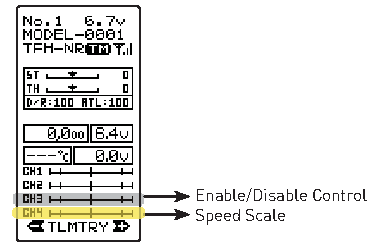
\includegraphics[width=1.0\linewidth]{futaba-screen.pdf}
  \caption{Futaba Radio Transmitter Screen}
  \label{futaba-screen}
\end{figure}

If you’re not seeing any action, check Contact on \autoref{contact} to get in touch with support.


\pagebreak[4]
\subsubsection{Body Lights}

Warthog includes eight RGB body lights, stacked in a pair on each corner of the chassis. These lights express system status according to \autoref{bodylights}, but in the absence of one of the low-level conditions, they can be commanded from ROS to display indications from autonomy or other higher-level software.

See \url{http://wiki.ros.org/warthog_base} for information on commanding the body lights.

\bgroup
\def\arraystretch{1.2}%
\begin{table}[h]
  \centering
  \begin{tabular}{>{\columncolor{lightgrey}}>{\raggedright}m{.25\textwidth} p{.7\textwidth}} \hline

  Solid red & The MCU is not in contact with the computer. That is, the rosserial connection is not active. This condition will be seen briefly on startup while Warthog's computer is booting up. If it persists, or is seen after initialization, either the base node on the PC has crashed, the network switch has failed, or a serious MCU error has occurred. If you suspect one of these conditions, please contact support. \\ \hline

  Red flashing & Stop circuit is broken. Twist the mushroom buttons to ensure that they are unlatched, and check any external stop hardware, if present. \\ \hline

  Alternating Red flashing and \\ Yellow corner flashing & All stops are closed but not reset, the stop loop is now only electrically latched. Press the stop reset button to enable full operation. \\ \hline

  Flashing yellow & Motor drivers not yet ready to drive. The motors have a brief initialization sequence which must complete after a stop condition clears before they are ready to drive. If this condition persists, please contact support. \\ \hline

  Headlights/taillights & When Warthog is ready to drive, the front will change from red to white. The intensity of the head and tail lights will increase slightly when actually in motion. This is the status which may be overridden by publishing your own light patterns to the cmd\_lights ROS topic. \\ \hline

  \end{tabular}
\newline
\caption{Warthog Body Light Indications}
\label{bodylights}
\end{table}
\egroup


\subsection{Wireless Access}

To connect to Warthog connect to one of the the network ports with a standard ethernet cable. Now, set your laptop’s ethernet port to a static IP such as \lstinline{192.168.131.51}, and connect via SSH to \lstinline{administrator@192.168.131.1}. The default password is \lstinline{clearpath}.

Additionally, you can connect to the Warthog's Access Point (AP) by setting a static IP as well. To do this in Ubuntu, follow the steps below:
\begin{enumerate}
  \item Click on the Wifi icon in the upper-right corner of your screen, and select \textbf{Edit Connections}
  \item In the \textbf{Network Connections} window, click \textbf{Add}, select \textbf{Wi-Fi},  and then click \textbf{Create}
  \item Fill out the \textbf{SSID} of the Warthog's AP as shown in Figure \autoref{wifi-ssid}
  \item Select the \textbf{Wi-Fi Security} tab and then change the \textbf{Security} to \lstinline{WPA & WPA2 Personal} as in Figure \autoref{wifi-security}
  \item Fill in the default password is \lstinline{clearpath}
  \item Select the \textbf{IPv4 Settings} tab and then change the \textbf{Method} to \lstinline{Manual} as detailed in Figure \autoref{wifi-ip}
  \item Click the \textbf{Add} button to add a new address
  \item Enter a \lstinline{192.168.131.51} as the static IP under the \textbf{Address} column, and enter \lstinline{255.255.255.0} under the \textbf{NetMask} column, and then select \textbf{Save}
\end{enumerate}

\begin{figure}[H]
  \centering
  \includegraphics[width=0.5\linewidth]{wifi-ssid.png}
  \caption{Static Wireless SSID Configuration}
  \label{wifi-ssid}
\end{figure}

\begin{figure}[H]
  \centering
  \includegraphics[width=0.5\linewidth]{wifi-security.png}
  \caption{Static Wireless Security Configuration}
  \label{wifi-security}
\end{figure}

\begin{figure}[H]
  \centering
  \includegraphics[width=0.5\linewidth]{wifi-ip.png}
  \caption{Static Wireless IP Configuration}
  \label{wifi-ip}
\end{figure}

\subsection{Remote ROS Connectivity}

Now that Warthog is on the wireless network, you can access it via SSH or as a remote ROS master. Note that in the default configuration, the background ROS process running on Warthog launches with the \lstinline{robot_upstart} package, which is configured to set the \lstinline{ROS_HOSTNAME} environment variable to the Warthog PC's hostname.

If your network resolves hostnames properly, connecting should be a matter of executing the following two lines in your desktop (or sourcing a script containing these lines):

\begin{lstlisting}
export ROS_MASTER_URI=http://cpr-warthog:11311     # Your robot's hostname
export ROS_IP=192.168.131.1                        # Your computer's wireless IP address
\end{lstlisting}

If your network doesn't resolve hostnames, you may need to add the following line to your \lstinline{/etc/hosts} file:

\begin{lstlisting}
192.168.131.1 cpr-warthog                         # The robot's wireless IP address.
\end{lstlisting}

Once everything is set up correctly, try running \lstinline{rostopic list}, which will verify that your machine can see the robot's ROS master, and \lstinline{rostopic echo /mcu/status}, which will verify that the robot PC can see your machine in order to stream topics to it.

Please contact Clearpath Support if guidance is required in selecting and executing a remote access strategy.
For more general details on how ROS works over TCP with multiple machines, please see:

\url{http://wiki.ros.org/ROS/Tutorials/MultipleMachines}

For help troubleshooting a multiple machines connectivity issue, see:

\url{http://wiki.ros.org/ROS/NetworkSetup}

\subsection{Visualizing Warthog}

To command or observe Warthog from your desktop computer, first set up a basic ROS installation.  See the following page for details:

\url{http://wiki.ros.org/indigo/Installation/Ubuntu}

When your ROS install is set up, install the Warthog desktop packages:

\begin{lstlisting}
sudo apt-get install ros-indigo-warthog-desktop
\end{lstlisting}

Once your remote access to Warthog's ROS master is configured (as above), you can launch rviz, the standard ROS robot visualization tool:

\begin{lstlisting}
roslaunch warthog_viz view_robot.launch
\end{lstlisting}

From within rviz, you can use interactive markers to drive Warthog, you can visulize its published localization estimate, and you can visualize any attached sensors which have been added to its robot description XML (URDF).

\pagebreak[4]

From your desktop, you can also launch the standard RQT Robot Monitor, which reports the diagnostic output from Warthog's self-monitoring capabilities, as shown in \autoref{robotmonitor}:

\begin{lstlisting}
rosrun rqt_robot_monitor rqt_robot_monitor
\end{lstlisting}

\begin{figure}[!htb]
  \centering
  \includegraphics[width=0.75\linewidth]{rqt_robot_monitor.png}
  \caption{Robot Monitor}
  \label{robotmonitor}
\end{figure}


\section{Safety Considerations}

Warthog is a powerful, heavy, fast moving robotic platform. Please read the following notices carefully.

\subsection{General Warnings}

Warthog is a rugged and high-performance vehicle. For the safety of yourself and others, always conduct initial experiments and software development with the motors not engaged.  Whenever the robot is not being operated and the motors are engaged, keep it in a stop state.  Do not ride of the vehicle, it can accelerate and brake quickley.

When starting out, favor slower wheel speeds. Warthog's control loops can accurately maintain velocities as low as 0.1 m/s. Operating at such speeds will give you more time to react if things don’t go quite as you expect.

\subsection{Maneuverability in Water}

Before entering the water it is important to ensure that:

\begin{itemize}[nolistsep]
  \item Bilge pumps are functioning properly
  \item The side panels and top cover are properly fastened down
  \item All Access panels are fastened down
\end{itemize}

Entrance and exit into the water should ideally be performed on a gradual incline to reduce the risk of flipping or taking on water. When entering the water, ensure that the Warthog UGV is driven in speed level 1. Once the Warthog UGV has entered the water the vehicle should be placed in speed level 3.

\subsection{Pinch Points}

When operating the Warthog UGV it is important to maintain a safe distance away from the unit. The suspension seen in Figure 3-5 has the ability to pivot.  Do not place fingers anywhere along the suspension link as it can result in injury.

\subsection{Stop Buttons}

The Stop system on the Warthog has three major components: The hardwired Stop switches, the Stop Reset button, and the wireless stop remote. Pressing down one of the 4 red, mushroom top buttons around the Warthog will disable power to the SEVCON devices (Key switch input on PIN 1). This disables the large contactors (shown in system electrical diagram) and also enables the brakes (passive, spring activated when not powered). The status indicator lights around the Warthog will flash red. To reset a Stop button, the top of the button should be twisted until the button pops out again. The status lights will then begin to scan red back and forth, with the lights on the rear right flashing yellow-red. This indicates that the Warthog is ready to be Stop reset. Pressing the red lit Stop Reset button (also indicated by the status panel flashing yellow-red) will fully enable the Warthog. The Warthog is fully enabled once a relay click is heard, and the front lights change to white.

To move the Warthog, the wireless remote stop also has to be powered on (by holding the Power button for at least 1 second). The remote Stop button toggles the Stop status, so must be pressed once to enable Stop, and pressed again to return to an Stop reset ready state, much like the hardwired Stop buttons. The reset button on the remote also behaves exactly like the onboard reset button. The wireless remote will shut itself off after 15 minutes of inactivity. Thus, the user is suggested to toggle the reset button (or either AUX 1 or 2) every few minutes to keep the remote awake. This is done to ensure that the user does not forget about the wireless remote, leading to a safety hazard.

Lastly, if either Stop Reset buttons (wired or wireless) are held down for more than 5 seconds, the computer is commanded to shut down via the MCU. This can be used to generate a proper shutdown for the computer, rather than a sudden power loss.

Always ensure the Stop button is accessible at all times. Avoid mounting payloads that extend over the rear of Warthog and would occlude the Stop buttons.

\subsection{Electrical System}

The largest electrical safety consideration with the Warthog system is the VBat connection. This is pulled straight from the batteries, it may have a voltage of 48V (depleted) - 62V (Charging) and can be used to power large external devices. This voltage can cause electrical shock if directly contacted, and is fused internally with an inline fuse at 20A. In general, take care to connect or disconnect devices preferably only when the entire system is powered off via the external switch on the rear (main power switch).

Included with the Warthog are several "dummy" connectors, to allow the user to keep unused connections securely blocked. Take note that triggering an Stop condition only disables voltage to the SEVCON drivers and motors, not the rest of the system which includes the connectors.  Please keep the "dummy" connectors attached unless an actual connector is attached.  Avoid working directly with the pins on the connector as it may short ciruit.

The labeled status LEDS on the user panels indicate status of the system voltages. If an LED is not lit, most likely a system fuse has blown, and contacting Clearpath is the best option.

To ensure saftey, please also observe the following precautions:

\begin{itemize}[nolistsep]
  \item Do not tamper with the battery terminals or wiring.
  \item Consult Clearpath Robotics support if you need to service the battery pack.
  \item Do not lay tools or other objects on top of the battery.
  \item Do not move the robot while charging the battery.
  \item Charge the battery only with the charger provided by Clearpath Robotics.
  \item Please dispose of the batteries properly, or return the batteries to Clearpath Robotics to do so.
\end{itemize}


\section{Payload Integration Guide}

If you want to attach custom hardware to Warthog, you will have to take care of mechnical mounting, electrical supply, and software integration.  This section aims to equip you with respect to these challenges.

\subsection{System Architecture}

Like most robotic systems, Warthog has an onboard PC coupled to a custom microcontroller board. The microcontroller board handles IO, system and battery monitoring, and provides an interface to the CAN-controlled motor drivers. See the diagram in \autoref{systemarchitecture} for more details.

\begin{figure}[!htb]
  \centering
  \includegraphics[width=1.0\linewidth]{warthog-logic-conn.pdf}
  \caption{System Architecture}
  \label{systemarchitecture}
\end{figure}

\pagebreak[4]
\subsection{Mechanical Mounting}
\label{mechanical}

The payload integration area can be used to mount external payloads on top of the Warthog.

\begin{figure}[!hbt]
  \centering
  \includegraphics[width=0.75\linewidth]{Payload_Integration_Plate.pdf}
  \caption{Warthog Payload Integration}
  \label{payloadplate}
\end{figure}

\subsubsection{Payload Integration Guidelines}

\begin{itemize}[nolistsep]

\item 27.75” is the maximum allowed width of any installed payload (this assumes that the payload is also centered across the width of the UGV chassis.

\item  No part of the payload may extend over the sheet metal housings of the drive units or into the small (~2”) gaps between the chassis and drive units. Damage to both the UGV and the payload WILL result.

\item  The chassis has a removable access cover measuring ~46.25” x 26.25”. This access cover is supported underneath by two adjustable cross members. Regardless of payload, it is imperative that both cross members remain installed (approximately evenly spaced) to provided required support to the access cover. Consider that any payload installed above the top deck will prevent access to the chassis through the access cover, without first removing the installed payload.

\item  The rotation of the suspension differential link in the horizontal plane will allow the payload to extend beyond the chassis top deck in both fore and aft locations. The amount of this payload extension (overhang) is dependent on several factors, including the weight and method of attachment of the payload as well as the terrain in which the UGV will operate. Ensure that the amount of overhanging payload allows the UGV to operate safely and doesn’t contact the terrain, especially when crossing steep and/or deep gullies.

\item  The available internal chassis volume is approximately 17.5” long x 26” wide x 9.5” high. This space is located at the center of the chassis between two battery packs. Consider that anything placed inside the chassis MUST be secured as to not move or shift during UGV operation. Any payload secured inside the chassis must also be insulated from coming into contact with the battery wiring and terminals.

\end{itemize}




\begin{warning}[]
Permanent damage resulting from custom modifications to the mounting plate is not covered under warranty and may not be supported by Clearpath Support.  Please contact our support team if you require assistance or have any questions relating to custom modifications.
\end{warning}


\pagebreak[4]
\subsection{Electrical Integration}
\label{electrical}

The three white Molex user power receptacles located in the User Bay are capable of supplying 5Vdc, 12Vdc, and unregulated battery voltage (approximately 24Vdc) for powering Warthog's payloads. See \autoref{userpower} for an labeled illustration and the pin assignments. The total draw permitted on each rail is 5A. The mating connector for these Molex Mini Fit Jr (tm) receptacles is \lstinline{39-01-2040}, available on Digikey as \lstinline{M3701-ND}. Ensure you select contact appropriate for the gauge of wire used.

\begin{figure}[!h]
  \centering
  \includegraphics[width=1.0\linewidth]{Warthog_UserPower_SOLID.pdf}
  \caption{Warthog Power User Panel}
  \label{userpower}
\end{figure}

The single red and black Anderson connector pair provides unregulated battery voltage (approximately 24Vdc) at up to 20-amps peak. The mating parts are Anderson PP45 Power Pole (tm) 1327 (red housing), 1327G6 (black housing) and 261G2-LPBK (contacts.) These components are readily available at \url{http://mouser.com}.

The rails on the User Bay Power board are protected against short circuit by fuses. See the illustration for the fuse locations and purposes.

\begin{warning}[Risk of Fire]
For continued protection against risk of fire, always replace fuses only with those of the same type and rating.
\end{warning}

\begin{warning}[Unregulated Rail]
The unregulated battery output may range from as low as 20Vdc up to 30Vdc or more depending on the state of charge of the battery pack and the electrical loading on the system. Ensure any accessories connected to that rail are able to deal with unregulated battery voltages.
\end{warning}


\subsection{Software Integration}

ROS has a large ecosystem of sensor drivers, some of which include pre-made URDF description and even simulation configurations.  Please see the following page on the ROS wiki for a partial list:

\url{http://wiki.ros.org/Sensors}

For the best experience, consider purchasing supported accessories from Clearpath Robotics for your Warthog, which will include simulation, visualization, and driver support.  However, we will happily help you get started with integrating your own devices as well.

\section{Maintenance}

\subsection{Battery \& Charging}

\subsubsection{General}

Warthog contains 48V lead-acid or lithium-ion battery packs. Each battery pack consists of four 12V leadacid or lithium-ion batteries.

Battery configuration may vary with each unit. In order to maximize performance it is important to ensure that the battery level across each set of lead-acid or lithium-ion batteries is within 0.1-0.2V of each other. If the battery packs exceed this tolerance, it is advised to charge them to within tolerance before wiring these packs
in parallel. The overall battery life will vary depending upon the usage of the unit.

Always exercise caution and observe the following safety practices connecting, disconnecting or handling batteries:

\begin{itemize}[nolistsep]
  \item Batteries are high voltage, high current
  \item Battery packs must be properly fastened down to ensure they do not move when the Warthog is in operation.
  \item Ensure that the battery packs are evenly distrubted throughout the Warthog to maximze stability.
  \item Battery levels on the unit should be checked on a regular basis.  It is important to maintain the battery voltage at a suitable level for proper operation.
  \item When additional battery packs are added to the system it is important to connect the positive terminal first to the main power of the Warthog before connecting ground.
  \item When installing additional battery packs, disconnect the ground on all battery packs presently in the unit before connecting the positive terminal of the new battery packs.
\end{itemize}

\subsubsection{Long-term Storage}

When storing Warthog for long periods of time, its important to properly maintain the batteries to fully maximize their life.  Consider one of the following two procedures when placing Warthog in long-term storage:

\begin{itemize}[nolistsep]
  \item Fully charge Warthog, turn it off and put it into storage.  Once a week, connect power to the charger and allow the charger to top up the battery for an hour or so.
  \item Fully charge Warthog, turn it off and put it into storage, but leave the charger connected and powered the enitre time Warthog is in storage.  The charger will monitor the battery and will automatically charge it up as needed.
\end{itemize}


Please contact Clearpath Robotics for additional information about Warthog's battery pack.


\section{Contact}
\label{contact}

Clearpath is committed to your success with Warthog. Please get in touch with us and we’ll do our best to get
you rolling again quickly: \url{support@clearpathrobotics.com}.

To get in touch with a salesperson regarding Warthog or other Clearpath Robotics products, please email
\url{sales@clearpathrobotics.com}.

If you have an issue that is specifically about ROS and is something which may be of interest to the broader
community, consider asking it on \url{answers.ros.org}. If you don’t get a satisfactory response, please ping us and
include a link to your question as posted there. If appropriate, we’ll answer in the ROS Answers context for
the benefit of the community.



\end{document}
